\documentclass[../../main.tex]{subfiles}
\begin{document}
In diesem Kapitel sei stets $K$ ein Körper.

\section{Matrixdarstellungen von linearen Abbildungen}

\begin{df}\label{7.1.1}
Seien $V$ und $W$ $K$-Vektorräume mit Basen [$\to$ \ref{6.2.1}(c), \ref{6.3.7}] $\underline{v} = (v_1,\ldots,v_n)$ und $\underline{w} = (w_1,\ldots,w_m)$. Eine Matrix $A\in K^{m\times n}$ heißt \emph{Darstellungsmatrix}\index{Matrix@{\bf Matrix}!Darstellungsmatrix} einer linearen Abbildung $f:V\to W$ bezüglich der Basen $\underline{v}$ und $\underline{w}$, falls [$\to$ \ref{6.3.2}(e)]
\begin{equation}\tag{$*$}
f = \ve_{\underline{w}}\circ f_A\circ \co_{\underline{v}}
\end{equation}
\begin{center}
\begin{tikzpicture}
\node(V){$V$};
\node[right = 2 of V](W){$W$};
\node[below = of V](Kn){$K^n$};
\node[below = of W](Km){$K^m$};

\draw[->, thick] (V) -- node[above]{$f$} (W);
\draw[->, thick] (Kn) -- node[below]{$x\mapsto Ax$} (Km);
\draw[->, thick] (Km) -- node[left]{$\cong$} node[right]{$\ve_{\underline{w}}$} (W);
\draw[->, thick] (V) -- node[right]{$\cong$} node[left]{$\co_{\underline{v}}$} (Kn);

\node[left = of V](sumlam){$\sum_{j=1}^{n}\lambda_jv_j$};
\node[below = .5 of sumlam](lam){$\cvec{\lambda_1\\\vdots\\\lambda_n}$};
\node[right = of W](summu){$\sum_{i=1}^{m}\mu_iw_i$};
\node[below = .5 of summu](mu){$\cvec{\mu_1\\\vdots\\\mu_m}$};

\draw[|->, thick] (sumlam) -- (lam);
\draw[|->, thick] (mu) -- (summu);
\end{tikzpicture}
\end{center}
\end{df}

\begin{bem}\label{7.1.2}
In der Situation von \ref{7.1.1} gilt
\begin{align*}
(*) & \overset{\ve_{\underline{w}}^{-1} = \co_{\underline{w}}}{\iff} \co_{\underline{w}}\circ f = f_A\circ \co_{\underline{v}}\\
& \overset{\ref{6.3.4}}\iff \forall j\in \left\{1,\ldots,n\right\}:\co_{\underline{w}}(f(v_j)) = \underbrace{f_A(\underbrace{\co_{\underline{v}}(v_j)}_{=e_j})}_{= Ae_j}\\
& \iff \forall j\in \left\{1,\ldots,n\right\}: Ae_j = \co_{\underline{w}}(f(v_j))
\end{align*}
\framebox{"`In den Spalten stehen die \textbf{Koordinaten der} Bilder der Basisvektoren."'}

\bigskip\noindent
Zu jeder linearen Abbildung zwischen endlichdimensionalen Vektorräumen gibt es also bezüglich gegebener Basen jeweils \emph{genau eine} Darstellungsmatrix.
\end{bem}

\begin{nt}\label{7.1.3}
$M(f,\underline{v},\underline{w})$ steht für das eindeutig bestimmte $A$ aus Definition \ref{7.1.1}.
\end{nt}

\begin{bsp}\label{7.1.4}
[$\to$ \ref{6.3.2}] $\underline{e} = (e_1,e_2) =\left(\cvec{1\\0},\cvec{0\\1}\right)$ Standardbasis des $\R^2$ [$\to$ \ref{6.2.2}].
\begin{enumerate}[\normalfont(a)]
\item $R_\ph :\R^2\to \R^2$ Drehung um $\ph$

\begin{minipage}{.5\textwidth}
\begin{align*}
& R_\ph (e_1) = \cvec{\cos \ph\\\sin\ph}\\
& R_\ph (e_2) = \cvec{-\sin\ph\\\cos\ph}\\
& R_\ph (e_1) = (\underline{\cos \ph})e_1 + (\underline{\sin\ph})e_2\\
& R_\ph (e_2) = (\underline{-\sin\ph})e_1 + (\underline{\cos\ph})e_2\\
& M(R_\ph, \underline{e},\underline{e}) = \begin{pmatrix}
\cos \ph & -\sin\ph\\
\sin \ph & \cos \ph
\end{pmatrix}
\end{align*}
\end{minipage}
\begin{minipage}{.4\textwidth}
\centering
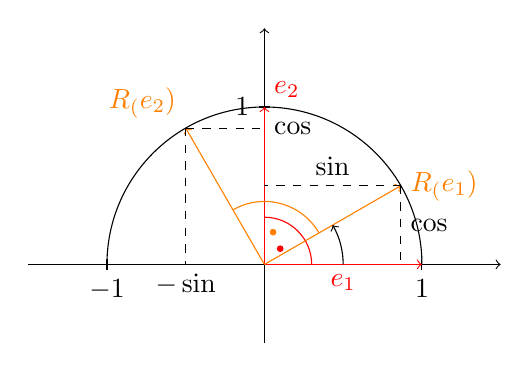
\begin{tikzpicture}[scale = 2]
\draw[->] (0,-.5) -- (0,1.5);
\draw[->] (-1.5,0) -- (1.5,0);

\draw (1,1pt) -- (1,-1pt) node[anchor = north]{$1$};
\draw (-1,1pt) -- (-1,-1pt) node[anchor = north]{$-1$};
\draw (1pt,1) -- (-1pt,1) node[anchor = east]{$1$};

\draw (1,0) arc (0:180:1);

\draw[->, red] (0,0) -- node[below]{$e_1$} (1,0);
\draw[->, red] (0,0) -- (0,1) node[anchor = south west]{$e_2$};
\draw[red] (.3,0) arc (0:90:.3);
\filldraw[red] (.1,.1) circle (.5pt);

\begin{scope}[rotate = 30]
\draw[->, orange] (0,0) -- (1,0) node[anchor = west]{$R_\ph(e_1)$};
\draw[->, orange] (0,0) -- (0,1) node[anchor = south east]{$R_\ph(e_2)$};
\draw[orange] (.4,0) arc (0:90:.4);
\filldraw[orange] (.15,.15) circle (.5pt);
\end{scope}

\draw[dashed] (.866,.5) -- node[right]{$\cos\ph$} (.866,0);
\draw[dashed] (.866,.5) -- node[above]{$\sin\ph$} (0,.5);
\draw[dashed] (-.5,.866) -- (0,.866) node[anchor = west]{$\cos\ph$};
\draw[dashed] (-.5,.866) -- (-.5,0) node[anchor = north]{$-\sin\ph$};

\draw[->] (.5,0) arc (0:30:.5);
\end{tikzpicture}
\end{minipage}
\item $S(e_1) = (\underline{-1})e_1+\underline{0}\cdot e_2$

$S(e_2) = \underline{0}e_1 + \underline{1}e_2$

$M (S,\underline{e},\underline{e}) = \begin{pmatrix}
-1 & 0\\
0 & 1
\end{pmatrix}$

$\underline{v} := \left(\cvec{0\\1},\cvec{1\\1}\right)$ und $\underline{w} := \left(\cvec{2\\1},\cvec{1\\-1}\right)$ sind auch
Basen des $\R^2$.
$$S(v_1) = S\cvec{0\\1} = \cvec{0\\1} = \frac{1}{3}\cvec{2\\1}+\left(-\frac{2}{3}\cvec{1\\-1}\right) = \frac{1}{3} w_1 + \left(-\frac{2}{3}\right) w_2$$
$$S(v_2) = S\cvec{1\\1} = \cvec{-1\\1} = 0\cvec{2\\1} + (-1) \cvec{1\\-1} = 0w_1 + (-1) w_2$$
$$M(S,\underline{v},\underline{w}) = \begin{pmatrix}
\frac{1}{3} & 0\\
-\frac{2}{3} & -1
\end{pmatrix}$$
\item $M(P,\underline{e},\underline{e}) = \begin{pmatrix}
1 & 0\\
0 & 0
\end{pmatrix}$, denn $P(e_1) = 1e_1+0e_2$ und $P(e_2) = 0e_1+0e_2$.
\item $M(T_a,\underline{e},\underline{e}) = \begin{pmatrix}
1 & a\\
0 & 1
\end{pmatrix}$, denn $T_a(e_1) = 1e_1+0e_2$ und $T_a(e_2) = ae_1+e_2$.
\item Schreibe $\underline{v}$ und $\underline{w}$ für die Standardbasen [$\to$ \ref{6.2.2}] des $K^n$ und $K^m$. Es gilt $\ve_{\underline{v}} = \id_{K^n}$ und $\ve_{\underline{w}} = \id_{K^m}$. Daher $\co_{\underline{v}} = \id^{-1}_{K^n} = \id_{K^n}$ und somit $f_A = \id_{K^m}\circ f_A\circ \id_{K^n} = \ve_{\underline{w}}\circ f_A\circ \co_{\underline{v}}$, das heißt $M(f_A,\underline{v},\underline{w}) = A$.
\item $\underline{v} := (1, X,\ldots,X^d)$ ist Basis von $K[X]_d$ [$\to$ \ref{6.2.8}(d)]
$$D^{(d)}(X^k) = \begin{cases}
0 & \text{falls } k = 0\\
kX^{k-1} &\text{falls }k\in \left\{1,\ldots,d\right\}.
\end{cases}$$
Also $M(D^{(d)},\underline{v},\underline{v}) = \begin{pmatrix}
0 & 1 & 0 & \cdots & 0\\
\vdots & 0 & 2 & \ddots & \vdots\\
\vdots & \vdots & 0 & \ddots & 0\\
\vdots & \vdots & \vdots & \ddots & d\\
 0 & 0 & 0 & \cdots & 0
\end{pmatrix}$, $D^{(d)}(X^2) = 2X = \underline{0}\cdot 1 + \underline{2}\cdot X+\underline{0}\cdot X^2+\ldots$
\item $\underline{v}$ wie eben, $\underline{w}:=$ Standardbasis des $K^n$.
$$E^{(d)}_{a_1,\ldots,a_n}(X^k) = \cvec{a_1^k\\\vdots\\a_n^k}$$
\begin{minipage}{.5\textwidth}
$M(E_{a_1,\ldots,a_n},\underline{v},\underline{w}) = \begin{pmatrix}
1 & a_1 & a_1^2 & \cdots & a_1^d\\
\vdots & \vdots & \vdots & & \vdots\\
1 & a_n & a_n^2 & \cdots & a_n^d
\end{pmatrix}$
\end{minipage}
\begin{minipage}{.425\textwidth}
\emph{Vandermonde}-Matrix\index{Matrix@{\bf Matrix}!Vandermonde-Matrix}

[\href{http://de.wikipedia.org/wiki/Alexandre-Théophile_Vandermonde}{Alexandre-Théophile Vandermonde}, *1735, \dag 1796]
\end{minipage}
\item $\underline{v} := (1,\i)$ ist Basis des $\R$-Vektorraums $\C$ [$\to$ \ref{6.2.8}(c)].

$$C(1) = \underline{1}\cdot1+\underline{0}\cdot \i,\quad C(\i) = \underline{0}\cdot1+(\underline{-1})\i$$
$$M(C,\underline{v},\underline{v}) = \begin{pmatrix}
1 & 0\\
0 & -1
\end{pmatrix}$$
$w := (1+\i, 1-\i)$ ist auch Basis des $\R$-Vektorraums $\C$.
$$C(1+\i) = 1-\i,\quad C(1-\i) = 1+\i$$
$$M(C,\underline{w},\underline{w}) = \begin{pmatrix}
0 & 1\\
1 & 0
\end{pmatrix}$$
$$C(1) = 1 = \underline{\frac{1}{2}}(1+\i) +\underline{\frac{1}{2}}(1-\i),\quad C(\i) = -\i = \underline{\left(-\frac{1}{2}\right)}(1+\i) + \underline{\frac{1}{2}}(1-\i)$$
$$M(C,\underline{v},\underline{w}) = \begin{pmatrix}
\frac{1}{2} & -\frac{1}{2}\\
\frac{1}{2} & \frac{1}{2}
\end{pmatrix}$$
$$C(1+\i) = \underline{1}\cdot 1 + \underline{(-1)}\i,\quad C(1-\i) = \underline{1}\cdot 1+\underline{1}\cdot \i$$
$$M(C,\underline{w},\underline{v})=\begin{pmatrix}
1 & 1\\
-1 & 1
\end{pmatrix}$$
\end{enumerate}
\end{bsp}

\begin{er}[Spezialfall von \ref{6.1.5}]\label{7.1.5}
Ist $I$ eine Menge und $V$ ein $K$-Vektorraum, so ist auch $V^I \overset{\text{\ref{1.1.27}}}{=}\left\{f\mid f:I\to V\right\}$ ein $K$-Vektorraum vermöge $(f+g)(i) = f(i) + g(i)$ und $(\lambda f)(i) = \lambda (f(i))$ für alle $f,g\in V^I$ und $\lambda\in K$.

Der Spezialfall $I= \left\{1,\ldots,m\right\}\times \left\{1,\ldots,n\right\}$ [$\to$ \ref{5.1.8}] und $V=K$ liefert den $K$-Vektorraum $K^{m\times n}$ der $m\times n$-Matrizen über $K$:
$$
\begin{pmatrix}
a_{11} & \cdots & a_{1n}\\
\vdots & & \vdots\\
a_{m1} & \cdots & a_{mn}
\end{pmatrix} + \begin{pmatrix}
b_{11} & \cdots & b_{1n}\\
\vdots & & \vdots\\
b_{m1} & \cdots & b_{mn}
\end{pmatrix} = \begin{pmatrix}
a_{11}+b_{11} & \cdots & a_{1n}+b_{1n}\\
\vdots & & \vdots\\
a_{m1}+b_{m1} & \cdots & a_{mn}+b_{mn}
\end{pmatrix}
$$
$$\lambda \begin{pmatrix}
a_{11} & \cdots & a_{1n}\\
\vdots & & \vdots\\
a_{m1} & \cdots & a_{mn}
\end{pmatrix} = \begin{pmatrix}
\lambda a_{11} & \cdots & \lambda a_{1n}\\
\vdots & & \vdots\\
\lambda a_{m1} & \cdots & \lambda a_{mn}
\end{pmatrix} \qquad (a_{ij}, b_{ij},\lambda\in K)$$
\end{er}

\begin{notpro}\label{7.1.6}
Sind $V$ und $W$ $K$-Vektorräume, so ist
$$\Hom(V,W) := \left\{f\mid f:V\to W \text{ linear}\right\}\index{Vektorraum@{\bf Vektorraum}!Homomorphismus/ lineare Abbildung!Hom@$\Hom(V,W)$}$$
ein Unterraum des $K$-Vektorraums $W^V$.
\end{notpro}
\begin{proof}
Nach \ref{6.1.10} ist zu zeigen:
\begin{enumerate}[\normalfont(a)]
\item $0\in \Hom(V,W)$ (wobei $0:V\to W, v\mapsto 0$)
\item $\forall f,g\in \Hom(V,W): f+g \in \Hom(V,W)$
\item $\forall f\in \Hom(V,W):\forall \mu\in K: \mu f\in \Hom(V,W)$
\end{enumerate}
\begin{enumerate}[Zu (a).]
\item $0 (v_1 +v_2) = 0_W = 0_W + 0_W = 0(v_1) + 0(v_2)$ für $v_1,v_2\in K$

$0(\lambda v) = 0_W = \lambda0_W = \lambda 0(v)$ für $v\in V$ und $\lambda\in K$
\item Seien $f,g:V\to W$ linear. Zu zeigen: $f+g$ linear.
\begin{align*}
(f+g)(v_1+v_2) & = f(v_1+v_2) + g(v_1+v_2) = f(v_1) + f(v_2) + g(v_1) + g(v_2)\\
& = f(v_1) + g(v_1) + f(v_2) + g(v_2) = (f+g)(v_1) + (f+g)(v_2)
\end{align*}
für alle $v_1,v_2\in V$
\begin{align*}
(f+g)(\lambda v) & = f(\lambda v) + g(\lambda v) = \lambda f(v) +\lambda g(v) = \lambda(f(v)+g(v)) = \lambda ((f+g)(v))
\end{align*}
für alle $v\in V$ und $\lambda\in K$.
\item Sei $f:V\to W$ linear und $\mu\in K$. Zu zeigen: $\mu f$ linear.
\begin{align*}
(\mu f)(v_1+v_2) & = \mu(f(v_1+v_2)) = \mu(f(v_1)+f(v_2)) = \mu(f(v_1)) + \mu(f(v_2))\\
& = (\mu f)(v_1) + (\mu f)(v_2)
\end{align*}
für alle $v_1,v_2\in V$
\begin{align*}
(\mu f)(\lambda v) & = \mu (f(\lambda v)) = \mu\lambda(f(v)) = \lambda \mu(f(v)) = \lambda ((\mu f)(v))
\end{align*}
für alle $v\in V$ und $\lambda\in K$.
\end{enumerate}
\end{proof}

\begin{exo}\label{7.1.7}
\begin{enumerate}[\normalfont(a)]
\item Sind $V$ und $W$ $K$-Vektorräume, $U\over{\xrightarrow{f}}{\xrightarrow[g]{}} V \xrightarrow{h}W$ Abbildungen, \emph{$h$ linear} und $\lambda\in K$, so
$$h\circ (f+g) = h\circ f+h\circ g\qquad \text{und} \qquad h\circ (\lambda f) = \lambda(h\circ f)$$
\item Sind $W$ ein $K$-Vektorraum, $U\xrightarrow{f}V\over{\xrightarrow{g}}{\xrightarrow[h]{}}W$ Abbildungen und $\lambda\in K$, so
$$(g+h)\circ f = g\circ f +h\circ f \qquad\text{und}\qquad (\lambda g)\circ f = \lambda(g\circ f)$$
\end{enumerate}
\end{exo}

\begin{sat}\label{7.1.8}
Seien $V$ und $W$ $K$-Vektorräume, $\underline{v} = (v_1,\ldots,v_n)$ eine Basis von $V$ und $\underline{w} = (w_1,\ldots,w_m)$ eine Basis von $W$.

Dann sind $\Phi : \begin{cases}
\Hom(V,W) \to K^{m\times n}\\
f\mapsto M(f,\underline{v},\underline{w})
\end{cases}$ und $\Psi : \begin{cases}
K^{m\times n} \to \Hom(V,W)\\
A\mapsto \ve_{\underline{w}} \circ f_A \circ \co_{\underline{v}}
\end{cases}$ zueinander inverse Vektorraumisomorphismen.
\end{sat}
\begin{proof}
Nach \ref{1.2.6} und \ref{6.3.3}(b) ist zu zeigen:
\begin{enumerate}[\normalfont(a)]
\item $\Phi \circ \Psi = \id_{K^{m\times n}}$
\item $\Psi \circ \Phi = \id_{\Hom(V,W)}$
\item $\Psi$ ist linear.
\end{enumerate}
\begin{enumerate}[Zu (a).]
\item Für $A\in K^{m\times n}$ gilt $(\Phi \circ \Psi)(A) = \Phi(\Psi(A)) = M(\ve_{\underline{w}}\circ f_A\circ \co_{\underline{v}}, v, w) \overset{\text{\ref{7.1.1}}}{\underset{\text{\ref{7.1.3}}}{=}} A$.
\item Für $f\in \Hom(V,W)$ gilt $(\Psi \circ \Phi)(f) = \ve_{\underline{w}} \circ f_{M(f,\underline{v},\underline{w})} \circ \co_{\underline{v}} \overset{\text{\ref{7.1.1}}}{\underset{\text{\ref{7.1.3}}}{=}} f$.
\item Seien $A,B \in K^{m\times n}$ und $\lambda\in K$.
\begin{align*}
\text{Zu zeigen: } & \ve_{\underline{w}} \circ f_{A+B} \circ \co_{\underline{v}} = \ve_{\underline{w}}\circ f_A \circ \co_{\underline{v}} + \ve_{\underline{w}} \circ f_B \circ \co_{\underline{v}}\\
\text{und } & \ve_{\underline{w}}\circ f_{\lambda A} \circ \co_{\underline{v}} = \lambda(\ve_{\underline{w}}\circ f_A \circ \co_{\underline{v}})
\end{align*}
Die rechten Seiten sind nach \ref{7.1.7} gleich
$$\ve_{\underline{w}}\circ (f_A+f_B) \circ \co_{\underline{v}} \qquad\text{und}\qquad \ve_{\underline{w}}\circ (\lambda f_A)\circ \co_{\underline{v}}.$$
Es reicht also $f_{A+B} = f_A + f_B$ und $f_{\lambda A} = \lambda f_A$ zu zeigen. Sei hierzu $x\in K^n$. Zu zeigen: $(A+B)x = Ax + Bx$ und $(\lambda A)x = \lambda (Ax)$. Dies rechnet man sofort nach.
\end{enumerate}
\end{proof}

\begin{kor}\label{7.1.9}
Sind $V$ und $W$ endlichdimensionale $K$-Vektorräume mit $n = \dim V$ und $m=\dim W$, so $\Hom(V,W)\cong K^{m\times n}$. Insbesondere gilt $\dim \Hom (V,W) = mn$.
\end{kor}

\begin{defbem}\label{7.1.10}
Sei $V$ ein $K$-Vektorraum mit Basen\\
$\underline{v} = (v_1,\ldots,v_n)$ und $\underline{w} = (w_1,\ldots,w_n)$. Dann heißt $M(\underline{v},\underline{w}):= M(\id_V,\underline{v},\underline{w})\in K^{n\times n}$ die \emph{Matrix des Basiswechsels}\index{Matrix@{\bf Matrix}!Darstellungsmatrix!Basiswechselmatrix} von $\underline{v}$ nach $\underline{w}$. Dies ist nach \ref{7.1.1} die eindeutig bestimmte Matrix $A\in K^{n\times n}$ mit $\co_{\underline{w}}  = f_A \circ \co_{\underline{v}}$. Sind also $\lambda_1,\ldots,\lambda_n$ die Koordinaten eines Vektors bezüglich $\underline{v}$, so sind $\mu_1,\ldots,\mu_n$ mit $\cvec{\mu_1\\\vdots\\\mu_n}:= M(\underline{v},\underline{w})\cvec{\lambda_1\\\vdots\\\lambda_n}$ die Koordinaten desselben Vektors bezüglich $\underline{w}$.
\end{defbem}

\begin{df}\label{7.1.11}
Ist $V$ ein $K$-Vektorraum mit Basis $\underline{v} = (v_1,\ldots,v_n)$ und $f: V \to V$ linear, so heißt $M(f,\underline{v}) := M(f,\underline{v},\underline{v})\in K^{n\times n}$ \emph{Darstellungsmatrix}\index{Matrix@{\bf Matrix}!Darstellungsmatrix} von $f$ bezüglich $\underline{v}$.
\end{df}

\red{Bis hierher sollten wir am 23. Dezember kommen.}

\section{Matrizenkalkül}

\begin{df}(auch gültig, wenn $K$ nur ein kommutativer Ring statt einem Körper ist!)\label{7.2.1}
Seien $m,n,r\in\N_0$, $A=(a_{ij})_{1\le i\le m,1\le j\le n}\in K^{m\times n},B=(b_{jk})_{1\le j\le n,1\le k\le r}\in K^{n\times r}$. Dann ist das \emph{Matrizenprodukt}\index{Matrix@{\bf Matrix}!Matrizenprodukt}
$AB=A\cdot B\in K^{m\times r}$ definiert durch
\[AB=\left(\sum_{j=1}^na_{ij}b_{jk}\right)_{1\le i\le m,1\le k\le r}.\]
Veranschaulichung: $\begin{pmatrix}
\tikz[baseline=(m1.base)]\node[draw=red, circle, inner sep = 2](m1){1}; & \tikz[baseline=(m2.base)]\node[draw=red, circle, inner sep = 2](m2){3}; & \tikz[baseline=(m3.base)]\node[draw=red, circle, inner sep = 2](m3){4};\\
-1 & 2 & 3\\
0 & 1 & 5\\
4 & 1 & 0
\end{pmatrix}\begin{pmatrix}
\tikz[baseline=(o1.base)]\node[inner sep = 2](o1){1}; & \tikz[baseline=(n1.base)]\node[draw=red, circle, inner sep = 2](n1){0};\\
\tikz[baseline=(o2.base)]\node[inner sep = 2](o2){5}; & \tikz[baseline=(n2.base)]\node[draw=red, circle, inner sep = 2](n2){1};\\
\tikz[baseline=(o3.base)]\node[inner sep = 2](o3){0}; & \tikz[baseline=(n3.base)]\node[draw=red, circle, inner sep = 2](n3){3};
\end{pmatrix} = \begin{pmatrix}
\tikz[baseline=(z1.base)]\node[fill=blue!20, circle, inner sep = 2](z1){16}; & \tikz[baseline=(z2.base)]\node[draw=red, circle, inner sep = 2](z2){15};\\
9 & 11\\
5 & 16\\
9 & 1
\end{pmatrix}
\begin{tikzpicture}[overlay]
\draw[opacity=.2,line width=5 mm,line cap=round,color=blue] (m1.center) to (m3.center);
\draw[opacity=.2,line width=5 mm,line cap=round,color=blue] (o1.center) to (o3.center);
\path (m1.north) edge [very thick,color=blue,bend left=40] (o1.north);
\path (m2.south) edge [very thick,color=blue,bend right=20] (o2.west);
\path (m3.south east) edge [very thick,color=blue,bend right=20] (o3.west);
\path (m1.north east) edge [very thick,color=red,bend left=40] (n1.north west);
\path (m2.north east) edge [very thick,color=red,bend left=40] (o1.west);
\path (o1.west) edge [very thick,color=red,bend right=20] (n2.west);
\path (m3.south) edge [very thick,color=red,bend right=45] (n3.south west);
\end{tikzpicture}$
\end{df}

\begin{bem}\label{7.2.2}
\begin{enumerate}[\normalfont(a)]
\item Ist $n=0$, so ist $AB=0\in K^{m\times r}$ die \emph{Nullmatrix}, aber $m,r\in\N_0$ können beliebig gewählt werden. Nur in diesem Ausnahmefall müsste man in die Notation
$A\cdot B$ eigentlich $m$ und $r$ aufnehmen, aber aus dem Zusammenhang ist ohnehin meist klar, was $m$ und $r$ sein sollen.
\item Damit das Matrixprodukt zweier Matrizen definiert ist, muss die erste Matrix genau so viele Spalten haben, wie die zweite Zeilen hat. Mit anderen Worten: Die Zeilen der ersten
Matrix müssen genauso lang sein, wie die Spalten der zweiten Matrix. Der Eintrag in der $i$-ten Zeile und $k$-ten Spalte von $AB$ ist dann das innere Produkt der $i$-ten Zeile
von $A$ mit der $k$-ten Spalte von $B$ ("`Zeile mal Spalte"'). Dabei nennt man $\sum_{i=1}^nx_iy_i$ für $x,y\in K^n$ das \emph{innere Produkt} von $x$ und $y$.
\item\label{sim}
Sind $x^{(1)},\dots,x^{(r)}$ die Spalten von $B$, so sind $Ax^{(1)},\dots,Ax^{(r)}$ die Spalten von $AB$:
\[A(x^{(1)}\dots x^{(r)})=(Ax^{(1)}\dots Ax^{(r)}).\]
Matrizenmultiplikation ist also "`simultanes Multiplizieren mit Spaltenvektoren"'.
\item
Sind $A\in K^{m\times n}$ und $x_1,\dots,x_n\in K$, so ist
\[A\underbrace{\begin{pmatrix}x_1\\\vdots\\x_n\end{pmatrix}}_{\in K^n}=A\underbrace{\begin{pmatrix}x_1\\\vdots\\x_n\end{pmatrix}}_{\in K^{n\times1}}.\]
\end{enumerate}
\end{bem}

\begin{bsp}\label{7.2.3}\mbox{}\\
\begin{enumerate}[\normalfont(a)]
\item
$
\begin{array}[t]{cccc}
\begin{pmatrix}1&0\\1&0\\2&1\end{pmatrix}&\begin{pmatrix}1&1&0&1\\1&1&0&0\end{pmatrix}&=&\begin{pmatrix}1&1&0&1\\1&1&0&1\\3&3&0&2\end{pmatrix}\\
\\
3\times\underline2&\underline2\times4&&3\times4
\end{array}
$
\item
$
\begin{array}[t]{cc}
\begin{pmatrix}1&1\\2&-1\end{pmatrix}&\begin{pmatrix}1&0\\1&1\\1&0\end{pmatrix}\\
\\
2\times\underline2&\underline3\times2
\end{array}
$ ist nicht definiert.
\item
$
\begin{array}[t]{cccc}
\begin{pmatrix}1&3&0&1\end{pmatrix}&\begin{pmatrix}0&1\\1&1\\-1&0\\0&2\end{pmatrix}&=&\begin{pmatrix}3&6\end{pmatrix}\\
\\
1\times\underline4&\underline4\times2&&1\times2
\end{array}
$
\end{enumerate}
\end{bsp}

\begin{lem}\label{7.2.4}
Seien $m,n,r\in\N_0$, $A\in K^{m\times n}$ und $B\in K^{n\times r}$. Dann gilt $f_{AB}=f_A\circ f_B$.
\end{lem}

\begin{proof}
Wegen $AB\in K^{m\times r}$ haben wir [$\to$ \ref{6.3.2} (e)]
\begin{center}
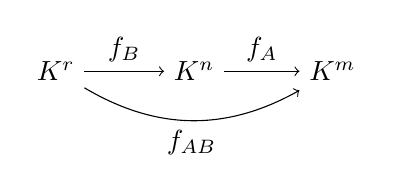
\begin{tikzpicture}[node distance=5em, auto]
  \node (1) {$K^r$};
  \node (2) [right of=1] {$K^n$};
  \node (3) [right of=2] {$K^m$};
  \draw[->] (1) to node {$f_B$} (2);
  \draw[->] (2) to node {$f_A$} (3);
  \draw[->,bend right] (1) to node [below] {$f_{AB}$} (3);
\end{tikzpicture},
\end{center}
so dass Definitions- und Zielmengen von $f_{AB}$ und $f_A\circ f_B$ übereinstimmen.
Da beide Abbildungen linear sind, reicht es nach \ref{6.3.4}, die Gleichheit auf den Standardvektoren [$\to$ \ref{6.2.2}]
$e_k\in K^r$ zu zeigen: Sei $k\in\{1,\dots,r\}$. Zu zeigen ist $(AB)e_k=A(Be_k)$. Da $Be_k$ die $k$-te Spalte von $B$ ist, ist $A(Be_k)$ nach \ref{7.2.2}\eqref{sim}
die $k$-te Spalte von $AB$, welche natürlich $(AB)e_k$ ist. 
\end{proof}

\begin{sat}\emph{("`Matrizenprodukt entspricht Hintereinanderschaltung von linearen Abbildungen"')}\label{7.2.5}
Seien $U,V,W$ $K$-Vektorräume der Dimensionen $r,n,m$ mit geordneten Basen $\u,\v,\w$. Seien
$U\overset g\longrightarrow V\overset f\longrightarrow W$ linear. Dann gilt $M(f\circ g,\u,\w)=M(f,\v,\w)M(g,\u,\v)$.
\end{sat}

\begin{proof}
Setzt man $A:=M(f,\underline v,\underline w)\in K^{m\times n}$, $B:=M(g,\u,\v)\in K^{n\times r}$, so ist $AB=M(f\circ g,\u,\w)$ zu zeigen, das heißt
$f\circ g=\ve_{\w}\circ f_{AB}\circ\co_\u$ [$\to$\ref{7.1.1}]. Nun gilt aber:
\begin{align*}
f\circ g&=(\ve_\w\circ f_A\circ\co_\v)\circ(\ve_\v\circ f_B\circ\co_\u)\\
&=\ve_\w\circ f_A\circ(\underbrace{\co_\v\circ\ve_\v}_{=\id_{K^n}})\circ f_B\circ\co_\u\\
&=\ve_\w\circ(f_A\circ f_B)\circ\co_\u\overset{\ref{7.2.4}}=\ve_\w\circ f_{AB}\circ\co_\u
\end{align*}
\end{proof}

\begin{kor}\emph{("`Matrizenmultiplikation ist assoziativ"')}\label{7.2.6}
Seien $m,n,r,s\in\N_0$, $A\in K^{m\times n}$, $B\in K^{n\times r}$ und $C\in K^{r\times s}$.
Dann gilt $(AB)C=A(BC)$.
\end{kor}

\begin{proof}
Bezeichne $\e^{(\ell)}$ die Standardbasis von $K^\ell$ für $\ell\in\N_0$. Dann gilt
\begin{align*}
(AB)C&=(M(f_A,\e^{(n)},\e^{(m)})M(f_B,\e^{(r)},\e^{(n)}))M(f_C,\e^{(s)},\e^{(r)})\\
&=M(f_A\circ f_B,\e^{(r)},\e^{(m)})M(f_C,\e^{(s)},\e^{(r)})\\
&=M((f_A\circ f_B)\circ f_C,\e^{(s)},\e^{(m)})\overset{\ref{1.2.5}(a)}=M(f_A\circ(f_B\circ f_C),\e^{(s)},\e^{(m)})\\
&=M(f_A,\e^{(n)},\e^{(m)})M(f_B\circ f_C,\e^{(s)},\e^{(n)})\\
&=M(f_A,\e^{(n)},\e^{(m)})(M(f_B,\e^{(r)},\e^{(n)})M(f_C,\e^{(s)},\e^{(r)}))=A(BC)
\end{align*}
\end{proof}

\begin{bem}\label{7.2.7}
\begin{enumerate}[\normalfont(a)]
\item
Man kann für Korollar \ref{7.2.6} auch den folgenden direkten Beweis geben, welcher zeigt, dass es auch richtig bleibt, wenn $K$ nur ein kommutativer Ring statt ein Körper ist:
Für $i\in\{1,\dots,m\}$ und $\ell\in\{1,\dots,s\}$ gilt
\begin{align*}
((AB)C)_{i\ell}&=\sum_{k=1}^r(AB)_{ik}C_{k\ell}\\
&=\sum_{k=1}^r\left(\sum_{j=1}^nA_{ij}B_{jk}\right)C_{k\ell}\\
&=\sum_{k=1}^r\sum_{j=1}^nA_{ij}B_{jk}C_{k\ell}\\
&=\sum_{j=1}^n\sum_{k=1}^rA_{ij}B_{jk}C_{k\ell}\\
&=\sum_{j=1}^nA_{ij}\sum_{k=1}^rB_{jk}C_{k\ell}\\
&=\sum_{j=1}^nA_{ij}(BC)_{j\ell}=(A(BC))_{i\ell}.
\end{align*}
\item Aus \ref{7.1.7} und \ref{7.1.8} folgt ähnlich wie im Beweis von \ref{7.2.6}, dass für alle $m,n,r\in\N_0$ gilt
\begin{align*}
&\forall A,B\in K^{m\times n}:\forall C\in K^{n\times r}:(A+B)C=AC+BC,\\
&\forall A\in K^{m\times n}:\forall B,C\in K^{n\times r}:A(B+C)=AB+AC&\text{und}\\
&\forall\la\in K:\forall A\in K^{m\times n}:\forall B\in K^{n\times r}:(\la A)B=\la(AB)=A(\la B).
\end{align*}
Dies kann man aber auch direkt nachrechnen und zwar sogar dann, wenn $K$ nur ein kommutativer Ring statt ein Körper ist, wobei man dann $\la A$ für $\la\in K$ und
$A\in K^{m\times n}$ analog zu \ref{7.1.5} "`eintragweise"' definiert (und $A+B$ für $A,B\in K^{m\times n}$ schon durch \ref{2.1.11} genauso wie in \ref{7.1.5} "`eintragweise"' definiert ist).
\item Wegen \ref{7.2.6} können wir beim Multiplizieren von mehreren Matrizen auf Klammern verzichten [$\to$\ref{2.1.7}].
\end{enumerate}
\end{bem}

\begin{bsp}\label{7.2.8}
Seien $\ph,\ps\in\R$. Dann $R_{\ph+\ps}=R_\ph\circ R_\ps$ aus geometrischen Gründen und mit \ref{7.2.5} daher
$M(R_{\ph+\ps},\e)=M(R_\ph,\e)M(R_\ps,\e)$, was mit \ref{7.1.4}(a) heißt
\begin{multline*}
\begin{pmatrix}\cos(\ph+\ps)&-\sin(\ph+\ps)\\\sin(\ph+\ps)&\cos(\ph+\ps)\end{pmatrix}=
\begin{pmatrix}\cos(\ph)&-\sin(\ph)\\\sin(\ph)&\cos(\ph)\end{pmatrix}
\begin{pmatrix}\cos(\ps)&-\sin(\ps)\\\sin(\ps)&\cos(\ps)\end{pmatrix}\\
\overset{\ref{7.2.5}}=
\begin{pmatrix}
(\cos\ph)(\cos\ps)-(\sin\ph)(\sin\ps)&-(\cos\ph)(\sin\ps)-(\sin\ph)(\cos\ps)\\
(\sin\ph)(\cos\ps)+(\cos\ph)(\sin\ps)&-(\sin\ph)(\sin\ps)+(\cos\ph)(\cos\ps)
\end{pmatrix}.
\end{multline*}
Es folgen die \emph{Additionstheoreme}
\begin{align*}
\cos(\ph+\ps)&=(\cos\ph)(\cos\ps)-(\sin\ph)(\sin\ps)\text{ und}\\
\sin(\ph+\ps)&=(\sin\ph)(\cos\ps)+(\cos\ph)(\sin\ps).
\end{align*}
\end{bsp}

\begin{defprop}(auch falls $K$ nur ein kommutativer Ring statt einem Körper)\label{7.2.9}
Für $n\in\N_0$ heißt
\[I_n:=
    \begin{pmatrix}
      1 & \multicolumn{2}{c}{\text{\kern 1em\smash{\raisebox{-1.5ex}{\Huge 0}}}} \\
      & \ddots &  \\
      \multicolumn{2}{c}{\text{\kern-1.5em\smash{\raisebox{0ex}{\Huge 0}}}} & 1
    \end{pmatrix}\in K^{n\times n}
    \]
die \emph{Einheitsmatrix}\index{Matrix@{\bf Matrix}!Einheitsmatrix} der Größe $n$. Falls $n$ aus dem Zusammenhang klar ist, schreibt man oft $I$ statt $I_n$.
Man überprüft sofort $\forall A\in K^{m\times n}:AI_n=A$ und $\forall B\in K^{n\times r}:I_nB=B$.
Eine Matrix $A\in K^{n\times n}$ heißt \emph{invertierbar} (falls $K$ ein Körper auch \emph{regulär}), wenn es ein $B\in K^{n\times n}$ gibt mit
\[AB=I_n=BA.\]
In diesem Fall ist $B$ eindeutig bestimmt (hat $B'$ dieselben Eigenschaften, so $B'=B'I_n=B'AB=I_nB=B$) und heißt die zu $A$ \emph{inverse}\index{Matrix@{\bf Matrix}!inverse Matrix} Matrix, in Zeichen
$A^{-1}$.
\end{defprop}

\begin{pro}\label{7.2.10}
Seien $V$ ein Vektorraum mit Basis $\v=(v_1,\dots,v_n)$ und $f\colon V\to V$ linear. Dann $M(f,\v)=I_n\iff f=\id_V$.
\end{pro}

\begin{proof}
$M(f,\v)=I_n\overset{\ref{7.1.1}}\iff f=\ve_\v\circ\underbrace{f_{I_n}}_{=\id_{K^n}}\circ\co_\v
\iff f=\underbrace{\ve_\v\circ\co_\v}_{\id_V}
$
\end{proof}

\begin{pro}\label{7.2.11}
Seien $V$ und $W$ $K$-Vektorräume mit Basen $\v=(v_1,\dots,v_n)$ und $\w=(w_1,\dots,w_n)$. Sei $f\colon V\to W$ linear. Dann ist $M(f,\v,\w)$ invertierbar genau dann,
wenn $f$ bijektiv ist, und in diesem Fall gilt \[M(f,\v,\w)^{-1}=M(f^{-1},\w,\v).\]
\end{pro}

\begin{proof}
Ist $f$ bijektiv, so gilt $f\circ f^{-1}=\id_W$ und $f^{-1}\circ f=\id_V$ nach \ref{1.2.5}(c), also
\begin{align*}
I_n&\overset{\ref{7.2.10}}=M(f\circ f^{-1},\w,\w)\overset{\ref{7.2.5}}=M(f,\v,\w) M(f^{-1},\w,\v)\text{ und}\\
I_n&\overset{\ref{7.2.10}}=M(f^{-1}\circ f,\v,\v)\overset{\ref{7.2.5}}=M(f^{-1},\w,\v) M(f,\v,\w),
\end{align*}
das heißt $M(f,\v,\w)$ ist invertierbar mit $M(f,\v,\w)^{-1}=M(f^{-1},\w,\v)$.
Sei nun umgekehrt $A:=M(f,\v,\w)$ invertierbar, etwa $B\in K^{n\times n}$ mit $AB=I_n=BA$. Dann gilt für $g:=\ve_\v\circ f_B\circ\co_\w\colon W\to V$ unter Beachtung von
$f\overset{\ref{7.1.1}}=\ve_\w\circ f_A\circ\co_\v$:
\[
g\circ f=\ve_\v\circ f_B\circ f_A\circ\co_\v=\id_V\text{ und }
f\circ g=\ve_\w\circ f_A\circ f_B\circ\co_\w=\id_W,
\]
da $f_B\circ f_A\overset{\ref{7.2.4}}=f_{BA}=f_{I_n}\overset{\ref{7.2.10}}=\id_{K^n}$ und $f_A\circ f_B\overset{\ref{7.2.4}}=f_{AB}=f_{I_n}\overset{\ref{7.2.10}}=\id_{K^n}$. Aus \ref{1.2.6} folgt, dass dann $f$ bijektiv ist.
\end{proof}

\begin{pro}\label{7.2.12}
Seien $V$ und $W$ endlichdimensionale $K$-Vektorräume derselben Dimension \emph{[$\to$\ref{6.2.24}]} und $f\colon V\to W$ linear. Dann gilt
\[\text{$f$ injektiv}\iff\text{$f$ bijektiv}\iff\text{$f$ surjektiv.}\]
\end{pro}

\begin{proof}
Wähle mit \ref{6.2.18} eine Basis $\v=(v_1,\dots,v_n)$ von $V$. Nach \ref{6.3.8} gilt:
\begin{align*}
\text{$f$ injektiv}&\iff\text{$f(v_1),\dots,f(v_n)$ linear unabhängig in $W$,}\\
\text{$f$ bijektiv}&\iff\text{$f(v_1),\dots,f(v_n)$ bilden Basis von $W$,}\\
\text{$f$ surjektiv}&\iff\text{$f(v_1),\dots,f(v_n)$ spannen $W$ auf.}
\end{align*}
Wegen $\dim W=n$ sind nach \ref{6.2.26} die rechts stehenden Bedingungen aber äquivalent.
\end{proof}

\begin{sat}\label{7.2.13}
Seien $A,B\in K^{n\times n}$. Dann $AB=I_n\iff BA=I_n$.
\end{sat}

\begin{proof}
Wegen Symmetrie reicht es zu "`$\implies$"' zu zeigen. Gelte hierzu $AB=I_n$. Dann $f_A\circ f_B\overset{\ref{7.2.4}}=f_{AB}=f_{I_n}\overset{\ref{7.2.10}}=\id_{K^n}$, woraus folgt,
dass $f_B$ injektiv ist. Aus \ref{7.2.12} folgt, dass $f_B$ bijektiv ist, woraus man mit \ref{7.2.11} die Invertierbarkeit von $B$ erhält. Es folgt
$$BA=BA(BB^{-1})=B(AB)B^{-1}=BB^{-1}=I_n.$$
\end{proof}

\begin{kor}\label{7.2.14}
Sei $A\in K^{n\times n}$. Dann ist $A$ invertierbar genau dann, wenn es \[x^{(1)},\dots,x^{(n)}\in K^n\] gibt mit $Ax^{(j)}=e_j$ für alle $j\in\{1,\dots,n\}$. In diesem Fall
sind $x^{(1)},\dots,x^{(n)}$ eindeutig bestimmt und $x^{(j)}$ ist die $j$-te Spalte von $A^{-1}$.
\end{kor}

\begin{proof}
Folgt direkt aus \ref{7.2.13} und \ref{7.2.2}\eqref{sim}.
\end{proof}

\noindent
Zur Berechnung von Matrixinversen, muss man also sogenannte \emph{inhomogene} lineare Gleichungssysteme lösen, was Gegenstand des nächsten Abschnitts ist.

\red{Bis hierher sollten wir am 10. Januar kommen.}

\section[tocentry={Inhomogene lineare Gleichungssysteme}]{Inhomogene lineare Gleichungssysteme {\small [$\to$ §\ref{5}]}}\label{7.3}

\begin{sprbem}\label{7.3.1}
[$\to$ \ref{5.1.1}, \ref{5.1.12}] Ein \emph{lineares Gleichungssystem} über $K$ ist (ggf. nach Umstellen) von der Form \[(*)\qquad Ax = b\quad (x\in K^n),\] wobei $A\in K^{m\times n}$ und $b\in K^m$ vorgegeben sind und $x\in K^n$ gesucht ist ($m$ Gleichungen in $n$ Unbekannten). Ist $b = 0$, so heißt $(*)$ \emph{homogen}, ansonsten \emph{inhomogen}\index{inhomogenes lineares Gleichungssystem@{\bf inhomogenes lineares Gleichungssystem}}. Der homogene Fall ist hier zugelassen, wurde aber schon in §\ref{5} behandelt. Ist $A$ in Stufenform\index{inhomogenes lineares Gleichungssystem@{\bf inhomogenes lineares Gleichungssystem}!Stufenform} [$\to$ \ref{5.1.10}], so nennen wir wieder für $j\in\left\{1,\ldots,n\right\}$ die Unbekannte $x_j$ \case{\emph{abhängig}}{\emph{frei}}\index{inhomogenes lineares Gleichungssystem@{\bf inhomogenes lineares Gleichungssystem}!Stufenform!abhängige Unbekannte}\index{inhomogenes lineares Gleichungssystem@{\bf inhomogenes lineares Gleichungssystem}!Stufenform!freie Unbekannte} in $(*)$, wenn $j$ \case{eine}{keine} Stufenposition [$\to$ \ref{5.1.10}] von $A$ ist. Ist $A$ sogar in \emph{reduzierter Stufenform}\index{inhomogenes lineares Gleichungssystem@{\bf inhomogenes lineares Gleichungssystem}!Stufenform!reduzierte Stufenform} mit $r$ Stufen und Stufenpositionen $j_1,\ldots,j_r$, so kann man offensichtlich $(*)$ als ein System von $m$ linearen Gleichungen
\[
\begin{split}
x_{j_1} & = b_1 + \ldots\\
& \ ~\vdots\\
x_{j_r} & =  b_r + \ldots\\
 0 & =  b_{r+1}\\
 & \ ~\vdots\\
 0 & =  b_m
\end{split}
\qquad(x\in K^n)
\]
schreiben, auf deren rechten Seiten nur freie Unbekannte auftauchen. Es sind nun zwei Fälle zu unterscheiden:
\begin{enumerate}[{Fall} 1:]
\item nicht $b_{r+1} = \ldots = b_m = 0$

Dann ist $(*)$ unlösbar (leere Lösungsmenge).
\item $b_{r+1} = \ldots = b_m = 0$

Dann existiert für jede Festlegung der freien Unbekannten wieder genau eine Wahl der abhängigen Unbekannten derart, dass $Ax = b$ gilt. Damit kann man dann unmittelbar $x^{(0)}, \xi^{(1)},\ldots, \xi^{(n-r)}\in K^n$ bestimmen mit
$$\left\{x\in K^n\mid Ax = b\right\} = \left\{x^{(0)}+\xi\mid \xi\in\spann{\xi^{(1)},\ldots,\xi^{(n-r)}}\right\}$$
\end{enumerate}
\end{sprbem}

\begin{bsp}\label{7.3.2}
[$\to$ \ref{5.1.13}] $K = \Q$
$$(*)\qquad \begin{array}{rrrrl}
x_1 & -3x_4 & + x_5 & +x_7 & = 1\\
& x_2 & -x_3 & +x_5 & = 2\\
& & x_6 & -x_7 & =-1
\end{array}\qquad (x_1,\ldots,x_7\in \Q)$$
$x_1,x_2,x_6$ abhängig, $x_3,x_4,x_5,x_7$ frei.
\begin{multline*}
\Set{x\in\Q^7 | \begin{array}{rrrrr}
x_1 = & 1 & +3x_4 & -x_5 & -x_7\\
x_2 = & 2 & +x_3 & -x_5\\
x_6 = & -1 & +x_7
\end{array}, x_3,x_4,x_5,x_7\in\Q}\\
 =\Set{\cvec{1+3x_4-x_5-x_7\\2+x_3-x_5\\x_3\\x_4\\x_5\\-1+x_7\\x_7} | x_3,x_4,x_5,x_7\in\Q}\\
= \Set{\cvec{1\\2\\0\\0\\0\\-1\\0}+x_3\cvec{0\\1\\1\\0\\0\\0\\0}+x_4\cvec{3\\0\\0\\1\\0\\0\\0}+x_5\cvec{-1\\-1\\0\\0\\1\\0\\0}+x_7\cvec{-1\\0\\0\\0\\0\\1\\1} | x_3,x_4,x_5,x_7\in \Q}
\end{multline*}
$$= \Set{\underbrace{\cvec{1\\2\\0\\0\\0\\-1\\0}}_{x_{(0)}}+\xi | \xi \in \spann{\underbrace{\cvec{0\\1\\1\\0\\0\\0\\0}}_{\xi^{(1)}},\underbrace{\cvec{3\\0\\0\\1\\0\\0\\0}}_{\xi^{(2)}},\underbrace{\cvec{-1\\-1\\0\\0\\1\\0\\0}}_{\xi^{(3)}},\underbrace{\cvec{-1\\0\\0\\0\\0\\1\\1}}_{\xi^{(4)}}}}$$
Keines der so berechneten $\xi^{(\ell)}$ ist überflüssig, denn ist $x_j$ eine freie Unbekannte, so gibt es im Fall 2 von \ref{7.3.1} eine Lösung von $(*)$ mit $x_j\ne0$
(etwa $x_j=1$) und eine solche Lösung bekommen wir nicht, ohne das zu $x_j$ gehörige $\xi^{(\ell)}$ zu benutzen, denn die $j$-te Komponente von $x^{(0)}$ und von
den anderen $\xi^{(k)}$ ist jeweils null.
\end{bsp}

\begin{bem}\label{7.3.3}
[$\to$ \ref{5.1.14}] \begin{enumerate}[\normalfont(a)]
\item Da man stets wie in \ref{7.3.2} vorgehen kann, ist geklärt, wie man lineare Gleichungssysteme
\[Ax = b\quad(x\in K^n)\]
mit \emph{Koeffizientenmatrix} $A\in K^{m\times n}$ in \emph{reduzierter Stufenform} und \emph{rechter Seite} $b\in K^m$ löst.
\item Im allgemeinen Fall schreibt man ein lineares Gleichungssystem so um, dass dessen Koeffizientenmatrix schließlich in \emph{reduzierter Stufenform} vorliegt. Dazu bildet man die \emph{erweiterte Koeffizientenmatrix} $(A\ b)\in K^{m\times (n+1)}$ und führt sie durch erlaubte Zeilenoperationen [$\to$ §\ref{5.2}] in eine Matrix
$(A'\ b')\in K^{m\times(n+1)}$ mit $A'$ in Stufenform über. Es gilt dann 
\begin{multline*}
\left\{x\in K^n\mid Ax = b\right\}  = \left\{x\in K^n\mid\cvec{x\\-1}\in\ker(A\ b)\right\}\\
 \overset{(A\ b)\sim(A'\ b')}{\underset{\mathclap{\ref{5.3.4}}}{=}}~~~~ \left\{x\in K^n\mid\cvec{x\\-1}\in\ker(A'\ b')\right\}= \left\{x\in K^n\mid A'x = b'\right\}.
\end{multline*}
Will man gleich mehrere lineare Gleichungssysteme mit derselben Koeffizientenmatrix aber verschiedenen rechten Seiten lösen, so kann man die Koeffizientenmatrix um mehrere rechte Seiten erweitern.
\end{enumerate}
\end{bem}

\begin{bsp}\label{7.3.4}
[$\to$ \ref{5.2.6}] $K = \F_5, 2:=1+1, 3 := 1+1+1$ usw.
$$A:=\begin{pmatrix}
0 & 4 & 1 & 3\\
2 & 3 & 2 & 1\\
1 & 2 & 3 & 4\\
2 & 4 & 1 & 3
\end{pmatrix}\in \F_5^{4\times 4},\quad b_1 :=\cvec{1\\1\\0\\0},\quad b_2:=\cvec{1\\0\\0\\0}$$
Um $\left\{x\in\F_5^{4}\mid Ax = b_i\right\}$ für $i\in\left\{1,2\right\}$ zu berechnen, bilden wir die erweiterte Koeffizientenmatrix $(A\ b_1\ b_2)\in \F_5^{4\times 6}$ und berechnen $A'\in \F_5^{4\times 4}$ in reduzierter Stufenform und $b_1',b_2'\in \F_5^4$ mit $(A\ b_1\ b_2)\sim (A'\ b_1'\ b_2')$.
\begin{multline*}
\left(\begin{array}{cccc|cc}
0 & 4 & 1 & 3 & 1 & 1\\
2 & 3 & 2 & 1 & 1 & 0\\
1 & 2 & 3 & 4 & 0 & 0\\
2 & 4 & 1 & 3 & 0 & 0
\end{array}\right) \overset{\over{\scriptstyle Z_1\leftrightarrow Z_3}{\scriptstyle Z_2\leftarrow Z_2-2Z_1}}{\underset{Z_4\leftarrow Z_4-2Z_1}{\sim}}\left(\begin{array}{cccc|cc}
1 & 2 & 3 & 4 & 0 & 0\\
0 & 4 & 1 & 3 & 1 & 0\\
0 & 4 & 1 & 3 & 1 & 1\\
0 & 0 & 0 & 0 & 0 & 0
\end{array}\right)\\
\overset{Z_3\leftarrow Z_3-Z_2}{\sim}\left(\begin{array}{cccc|cc}
1 & 2 & 3 & 4 & 0 & 0\\
0 & 4 & 1 & 3 & 1 & 0\\
0 & 0 & 0 & 0 & 0 & 1\\
0 & 0 & 0 & 0 & 0 & 0
\end{array}\right)
\overset{Z_2\leftarrow\frac{1}{4}Z_2}{\sim} \left(\begin{array}{cccc|cc}
1 & 2 & 3 & 4 & 0 & 0\\
0 & 1 & 4 & 2 & 4 & 0\\
0 & 0 & 0 & 0 & 0 & 1\\
0 & 0 & 0 & 0 & 0 & 0
\end{array}\right)\\
\overset{Z_1\leftarrow Z_1-2Z_2}{\sim} \left(\begin{array}{cccc|cc}
\tikz[baseline=(m1.base)]\node(m1){$1$}; & 0 & 0 & 0 & 2 & 0\\
0 & \tikz[baseline=(m2.base)]\node(m2){$1$}; & 4 & \tikz[baseline=(m3.base)]\node(m3){$2$}; & 4 & 0\\
0 & 0 & 0 & 0 & 0 & 1\\
\tikz[baseline=(m4.base)]\node(m4){$0$}; & 0 & 0 & \tikz[baseline=(m5.base)]\node(m5){$0$}; & 0 & 0
\end{array}\right)
\begin{tikzpicture}[overlay]
\draw (m1.north west) -- (m1.south west) -- (m2.north west) -- (m2.south west) -- (m3.south east);
\draw[decorate,decoration={brace,mirror},thick] ([yshift=-0.5em]m4.south west) -- node[anchor=north]
{$\substack{\text{Stufenform, 2 Stufen, Stufenpositionen $1,2$}\\\text{abhängig: $x_1,x_2$, frei: $x_3,x_4$}}$} ([yshift=-0.5em]m5.south east);
\end{tikzpicture}
\end{multline*}

\vspace{3em}
$$\left\{x\in \F_5^4\mid Ax = b_2\right\} = \emptyset$$
\begin{align*}
\left\{x\in \F_5^4\mid Ax = b_1\right\} & = \Set{\cvec{2\\4-4x_3-2x_4\\x_3\\x_4} | x_3,x_4\in \F_5}\\
& = \Set{\cvec{2\\4\\0\\0}+\xi | \xi\in \spann{\cvec{0\\1\\1\\0},\cvec{0\\3\\0\\1}}}
\end{align*}
Mit \ref{7.2.14} kann man so auch Matrixinverse berechnen.
\end{bsp}

\begin{sat}\label{7.3.5}
Seien $A,B,S\in K^{n\times n}$ mit $(A~I_n)\sim (S~B)$ und $S$ in reduzierter Stufenform. Dann ist $A$ invertierbar {\rm[$\to$ \ref{7.2.9}]} genau dann, wenn $S = I_n$ gilt. In diesem Fall gilt $B = A^{-1}$.
\end{sat}
\begin{proof}
Zu zeigen:
\begin{enumerate}[\normalfont(a)]
\item $S \ne I_n \Longrightarrow A$ nicht invertierbar
\item $S = I_n \Longrightarrow (A \text{ invertierbar }\et A^{-1}=B)$
\end{enumerate}
Bezeichne $b_j$ die $j$-te Spalte von $B$ für $j\in \left\{1,\ldots,n\right\}$. Aus $(A~I_n)\sim(S~B)$ folgt $(A~e_j) \sim (S~b_j)$ für $j\in \left\{1,\ldots,n\right\}$.
\begin{enumerate}[Zu (a).]
\item Gelte $S\ne I_n$. Dann gilt $n\ge 1$. Wegen $(A~e_1)\sim (S~b_1)$ gilt $\left\{x\in K^n\mid Ax = e_1\right\} = \left\{x\in K^n\mid Sx = b_1\right\}$. Da $S$ in reduzierter Stufenform ist, hat $S\in K^{n\times n}$ höchstens $n-1$ Stufen und das Gleichungssystem $Sx = b_1 \quad (x\in K^n)$ mindestens eine freie Variable [$\to$ \ref{7.3.1}]. Daher gibt es \emph{kein} oder \emph{mehrere} $x^{(1)}\in K^n$ mit $Ax^{(1)} = e_1$, je nachdem ob in \ref{7.3.1} Fall 1 oder 2 eintritt. Wäre $A$ invertierbar, so stünde dies im Widerspruch zu \ref{7.2.14}.
\item Gelte $S = I_n$. Dann gilt $\left\{x\in K^n\mid Ax = e_j\right\} = \left\{x\in K^n\mid I_nx = b_j\right\} = \left\{b_j\right\}$ und insbesondere $Ab_j = e_j$ für $j\in \left\{1,\ldots,n\right\}$. Nach \ref{7.2.14} ist $A$ invertierbar und $b_j$ die $j$-te Spalte von $A^{-1}$, das heißt $A^{-1} = B$.
\end{enumerate}
\end{proof}

\begin{bsp}\label{7.3.6}
$K = \R$.

Ist $\cvec{
1 & 2\\
-1 & 3
}$ invertierbar? Wenn ja, was ist das Inverse?
\begin{align*}
\left(\begin{array}{cc|cc}
1 & 2 & 1 & 0\\
-1 & 3 & 0 & 1
\end{array}\right) & \overset{Z_2 \leftarrow Z_2+ Z_1}{\sim} \left(\begin{array}{cc|cc}
1 & 2 & 1 & 0\\
0 & 5 & 1 & 1
\end{array}\right) \overset{Z_2\leftarrow \frac{1}{5}Z_2}{\sim}\left(\begin{array}{cc|cc}
1 & 2 & 1 & 0\\
0 & 1 & \frac{1}{5} & \frac{1}{5}
\end{array}\right)\\
&\overset{Z_1\leftarrow Z_1-2Z_2}{\sim} \left(\begin{array}{cc|cc}
1 & 0 & \frac{3}{5} & -\frac{2}{5}\\
0 & 1 & \frac{1}{5} & \frac{1}{5}
\end{array}\right).
\end{align*}
Also ist $\cvec{
1 & 2\\
-1 & 3
}$ invertierbar und $\cvec{
1 & 2\\
-1 & 3
}^{-1} = \frac{1}{5}\cvec{
3 & -2\\
1 & 1
}$.
\end{bsp}
\end{document}